\documentclass[t,xcolor={svgnames,table}]{beamer}

\mode<presentation>
\usetheme{Warsaw}
\useoutertheme{infolines} 

\usepackage{fontspec}
\usepackage{lmodern}
\usepackage{amsmath}
\usepackage{amsfonts}
\usepackage{bbm}
\usepackage{bm}
\usepackage[font=small,labelfont=bf]{caption} % Required for specifying captions to tables and figures
\usepackage{nicefrac}
\usepackage{color}
\usepackage{perpage}
\usepackage{multirow}
\usepackage{multicol}
\usepackage{adjustbox}
\usepackage{tikz}
\usepackage{tikz-dependency}
\usepackage{tikz-qtree}
\usepackage{tikz,pgfplots,pgfplotstable}
\usepackage{pgf}
\usepackage{collcell}
\usepackage{booktabs}
\usepackage{color,soul}

\usetikzlibrary{arrows.meta,graphs,graphs.standard,graphdrawing,quotes,shapes}
\usegdlibrary{layered,trees}

\tikzset{
  invisible/.style={opacity=0},
  visible on/.style={alt={#1{}{invisible}}},
  alt/.code args={<#1>#2#3}{%
    \alt<#1>{\pgfkeysalso{#2}}{\pgfkeysalso{#3}} % \pgfkeysalso doesn't change the path
  },
}

\captionsetup{labelformat=empty}
\newcommand{\parser}[1]{TUPA\textsubscript{#1}}

\newfontfamily\hebfont[Script=Hebrew, Scale=MatchUppercase]{FreeSans}
\newcommand{\heb}[1]{\bgroup\textdir TRT\hebfont #1\egroup}

\newcommand{\ucca}[1]{\textcolor{gray}{\textbf{\textsf{#1}}}}
\newcommand{\sst}[1]{\textsc{#1}}
\newcommand{\lexcat}[1]{\textsl{#1}}

\definecolor{orange}{rgb}{1,0.5,0}
\definecolor{mdgreen}{rgb}{0.05,0.6,0.05}
\definecolor{Acolor}{HTML}{EC5D57} % poppy red
\definecolor{Pcolor}{HTML}{70BF41} % grass green
\definecolor{Scolor}{HTML}{51A7F9} % sky blue
\definecolor{Lcolor}{HTML}{B36AE2} % friendly purple
\definecolor{mdblue}{rgb}{0,0,0.7}
\definecolor{dkblue}{rgb}{0,0,0.5}
\definecolor{dkgray}{rgb}{0.3,0.3,0.3}
\definecolor{slate}{rgb}{0.25,0.25,0.4}
\definecolor{gray}{rgb}{0.5,0.5,0.5}
\definecolor{ltgray}{rgb}{0.7,0.7,0.7}
\definecolor{purple}{rgb}{0.7,0,1.0}
\definecolor{lavender}{rgb}{0.65,0.55,1.0}


\makeatletter
\pgfdeclareshape{vector}{
      \inheritsavedanchors[from={rectangle}]
      \inheritbackgroundpath[from={rectangle}]
      \inheritanchorborder[from={rectangle}]
      \foreach \x in {center,north east,north west,north,south,south east,south west,east,west}{
        \inheritanchor[from={rectangle}]{\x}
      }

    \backgroundpath{
      \pgftransformshift{\pgfpoint{-16pt}{-4pt}}
          \draw[rounded corners=2pt] (0,0) rectangle (32pt,8pt);
    }

    \beforebackgroundpath{
      \draw[step=8pt,help lines,-] (8pt,.1pt) grid (24pt,7.9pt);
    }
}
\pgfdeclareshape{vector}{
      \inheritsavedanchors[from={rectangle}]
      \inheritbackgroundpath[from={rectangle}]
      \inheritanchorborder[from={rectangle}]
      \foreach \x in {center,north east,north west,north,south,south east,south west,east,west}{
        \inheritanchor[from={rectangle}]{\x}
      }

    \backgroundpath{
      \pgftransformshift{\pgfpoint{-16pt}{-4pt}}
          \draw[rounded corners=2pt] (0,0) rectangle (32pt,8pt);
    }

    \beforebackgroundpath{
      \draw[step=8pt,help lines,-] (8pt,.1pt) grid (24pt,7.9pt);
    }
}
\makeatother


% for confusion matrix
\newcommand{\ApplyGradient}[1]{%
  \pgfmathsetmacro{\PercentColor}{(#1-0)/63.88}%
  \pgfmathsetmacro{\PercentInverse}{ifthenelse(\PercentColor > 70, 0, 100)}%
  %\textcolor{black!\PercentColor}{#1}
  \edef\x{\noexpand\cellcolor{red!\PercentColor}}\x\textcolor{black!\PercentInverse}{#1}%
}
\newcolumntype{R}{>{\collectcell\ApplyGradient}{c}<{\endcollectcell}}


\MakePerPage{footnote}

% Outline slides
\AtBeginSection[]
{\begin{frame} \frametitle{Outline} \tableofcontents[currentsection,currentsubsection] \end{frame}}


\begin{document}


\title[]{Universal Meaning Representation Parsing}
\author{Daniel Hershcovich}
\date{ML Section Meeting \\ November 18, 2019}

\begin{frame}
\titlepage
\end{frame}

\begin{frame}
\frametitle{What can we do with Natural Language Processing?}
\onslide<2>{Machine translation:}
\begin{center}
\onslide<2,5>{
  \fbox{\heb{דניאל עבר לקופנהגן אחרי שסיים את הלימודים}}
}

\only<2,4>{
  \fbox{After graduation, Daniel moved to Copenhagen}
}
\only<3,5->{
  \fbox{After graduation, \underline{Daniel} moved to \underline{Copenhagen}}
}
\end{center}

\vspace{-7mm}
  
\only<3>{
  \vspace{-9mm}

  Named \\ entity \\ recognition:

  \hspace{54mm} $\downarrow$ \hspace{27mm} $\downarrow$

  \hspace{49mm} Person \hspace{17mm} Location
}

\only<4>{
  Text \\
  simplification:
}
  
\only<4->{
  \vspace{1mm}
  \begin{center}  
  \fbox{Daniel graduated. Then Daniel moved to Copenhagen.}
  \end{center}
}

\only<5->{
  Neural models require the right \textit{inductive bias} for tasks
  \cite{barrett-etal-2018-sequence,strubell-etal-2018-linguistically}.

  \begin{center}
    \begin{tikzpicture}[->]
    \tikzstyle{main}=[circle, minimum size=7mm, draw=black!80, node distance=12mm]
    \foreach \i in {1,3,7,9} {
        \node[main, fill=white!100] (h\i) at (\i,0) {};
        \node[main, fill=white!100] (o\i) at (\i.5,2) {};
    }
    \node (h5) at (5.5,0) {$\ldots$};
    \node (o5) at (5.5,2) {$\ldots$};
    \foreach \current/\next in {1/3,3/5,5/7,7/9} {
        \path (h\current) edge (h\next);
        \path (o\current) edge (o\next);
    }
    \foreach \i in {1,3,7,9} {
      \foreach \j in {1,3,7,9} {
        \path[gray!50] (h\i) edge (o\j);
      }
    }
    \end{tikzpicture}
  \end{center}
}

\end{frame}

\begin{frame}
\frametitle{Structured Inductive Bias}
Symbolic relations between words or concepts.

\vfill

Example: {\color{DarkBlue}syntactic}/{\color{DarkRed}semantic} bi-lexical dependencies.

\vfill

    \begin{adjustbox}{center}
    \begin{dependency}[line width=1.5pt]
        \begin{deptext}[column sep=1.5em,ampersand replacement=\^,font=\rmfamily]
          After \^ graduation \^ , \^ Daniel \^ moved \^ to \^ Copenhagen \\
        \end{deptext}
        \depedge[edge below,draw=DarkRed,edge unit distance=3ex]{1}{2}{ARG2}
        \depedge[edge below,draw=DarkRed,edge unit distance=3ex]{5}{4}{ARG1}
        \depedge[edge below,draw=DarkRed,edge unit distance=2ex, edge end x offset=-2pt]{1}{5}{ARG1}
        \deproot[edge below,draw=DarkRed,edge unit distance=3ex]{5}{top}
        \depedge[edge below,draw=DarkRed,edge unit distance=4ex, edge start x offset=-1pt, edge end x offset=3pt]{5}{7}{ARG2}
        \depedge[edge below,draw=DarkRed,edge unit distance=3ex, edge end x offset=5pt]{6}{5}{ARG1}
        \depedge[edge below,draw=DarkRed,edge unit distance=3ex]{6}{7}{ARG2}
        \depedge[draw=DarkBlue,edge unit distance=3ex]{2}{1}{case}
        \depedge[draw=DarkBlue,edge unit distance=3ex]{2}{3}{punct}
        \depedge[draw=DarkBlue,edge unit distance=3ex]{5}{4}{nsubj}
        \depedge[draw=DarkBlue,edge unit distance=3ex, edge end x offset=-2pt]{5}{2}{obl}
        \depedge[draw=DarkBlue,edge unit distance=3ex]{7}{6}{case}
        \deproot[draw=DarkBlue,edge unit distance=4ex]{5}{root}
        \depedge[draw=DarkBlue,edge unit distance=4ex]{5}{7}{obl}
    \end{dependency}    
    
    \end{adjustbox}
\end{frame}

\begin{frame}
    \frametitle{Meaning Representation}
Abstract away from detail that does not affect meaning:
\begin{center}    
    \fbox{\textrm{graduation}} $\approx$ \fbox{\textrm{graduated}}
    $\approx$ \fbox{\heb{סיים את הלימודים}} $\approx$ \fbox{\textrm{Abschluss}}
\end{center}

\pause\vfill

But capture useful distinctions, such as:
\vfill

\begin{minipage}{.38\textwidth}
\begin{itemize}
\item {\only<2>{\color{red}}Scenes and participants}
\item {\only<3>{\color{red}}Scene linkage}
\item {\only<4>{\color{red}}Multi-word chunking}
\end{itemize}
\end{minipage}
\begin{minipage}{.58\textwidth}\scalebox{.8}{
            \begin{tikzpicture}[level distance=21mm, sibling distance=1mm,
                every node/.append style={font=\rmfamily},
            	every circle node/.append style={fill=Indigo}]
                \begin{scope}[frontier/.style={distance from root=56mm},
                    edge from parent/.append style={nodes={font=\scriptsize}}]
                \Tree [.\node [circle] (root u) {};
                  \edge node[auto=right]{L}; \node[alt=<3>{text=red}{}] {Nach};
                  \edge node[auto=left]{H};
                  [.\node[circle](abschluss) {};
                    \edge node[auto=left]{P};
                    [.\node [circle] {};
                      \edge node[auto=right]{R}; \node {seinem};
                      \edge node[right]{C}; \node[alt=<2>{text=red}{}] (graduation) {Abschluss};
                    ]
                  ]
                  \edge node[auto=left]{H};
                  [.\node[circle]{};
                    \edge node[auto=left]{P};
                    [.\node[circle,xshift=8mm](zogum) {};
                      \edge node[auto=right]{}; \node[alt=<4>{text=red}{}] {zog};
                    ]
                    \edge node[auto=right]{A}; \node[alt=<2>{text=red}{}] (Daniel) {Daniel};
                    \edge[draw=none]; \node[alt=<4>{text=red}{}] (um) {um};
                  ]
                ]
                \draw[dashed] (abschluss) to node[auto] {\scriptsize A} (Daniel);
                \draw (zogum.south) to node[auto] {} (um);
                \end{scope}
            \end{tikzpicture}}
\end{minipage}\end{frame}


\section{UCCA}

\begin{frame}
\frametitle{Universal Conceptual Cognitive Annotation (UCCA)}
Supports rapid and intuitive annotation of linguistic semantic phenomena. \\
\only<1>{\cite{abend2013universal}}
\onslide<2->{
  Cross-linguistically applicable and stable \cite{sulem2015conceptual}.
}

\vfill

\begin{adjustbox}{center}
            \begin{tikzpicture}[level distance=7mm, sibling distance=6mm,
                every node/.append style={font=\rmfamily},
            	every circle node/.append style={fill=Indigo}]
                \begin{scope}[frontier/.style={distance from root=23mm},
                    edge from parent path={(\tikzparentnode.center)
                	.. controls +(0,-.25) and +(0,.25) .. (\tikzchildnode.north)},
                    edge from parent/.append style={nodes={font=\scriptsize}}]
                \Tree [.\node [circle] (root u) {};
                  \edge node [auto=right]{L}; \node (After u) {After};
                  \edge node[auto=left]{H};
                  [.\node [circle,xshift=8mm](graduation Daniel u) {};
                    \edge node[auto=right]{P}; \node (graduation u) {graduation};
                  ]
                  \edge node[auto=left]{H};
                  [.\node [circle](Daniel moved to Copenhagen u) {};
                    \edge node[auto=right]{A}; \node (Daniel u) {Daniel};
                    \edge node[auto=left]{P}; \node (moved u) {moved};
                    \edge node[auto=left]{A};
                    [.\node [circle](to Copenhagen u) {};
                      \edge node[auto=right]{R}; \node (to u) {to};
                      \edge node[auto=left]{C}; \node (Copenhagen u) {Copenhagen};
                    ]
                  ]
                ]
                \draw[dashed] (graduation Daniel u) to node[auto] {\scriptsize A} (Daniel u);
                \end{scope}
                \onslide<2->{
                  \begin{scope}[xshift=2cm,yshift=-58mm,grow'=up,level distance=9mm,
                      sibling distance=4mm, frontier/.style={distance from root=19mm},
                      edge from parent path={(\tikzparentnode.center) ..
                      controls +(0,.25) and +(0,-.25) .. (\tikzchildnode.south)},
                      edge from parent/.append style={nodes={font=\scriptsize}}]
                  \Tree [.\node [circle] (rootd) {};
                    \edge node[auto=left]{H};
                    [.\node [circle,xshift=-5mm] (Daniel siyem et halimudim d) {};
                      \edge node[auto=left]{P}; \node (halimudim d) {\heb{הלימודים}};
                      \edge node[auto=left]{F}; \node (et d) {\heb{את}};
                      \edge node[auto=right]{D}; \node (siyem d) {\heb{שסיים}};
                    ]
                    \edge node [auto=left,anchor=south east]{L}; \node (ahrei d) {\heb{אחרי}};
                    \edge node[auto=right]{H};
                    [.\node [circle] (hu avar lecopenhagen d) {};
                      \edge node[auto=left,anchor=south east]{A}; \node (lecopenhagen d) {\heb{לקופנהגן}};
                      \edge node[auto=left]{P}; \node (avar d) {\heb{עבר}};
                      \edge node[auto=right]{A}; \node (Daniel d) {\heb{דניאל}};
                    ]
                  ]
                  \draw[dashed] (Daniel siyem et halimudim d) to[out=-15,in=-150] node[above] {\scriptsize A} (Daniel d);
                  \end{scope}
                }\onslide<3>{
                  \begin{scope}[dashed,thick]
                    \draw[DarkRed] (After u) to[out=-45,in=135] (ahrei d);
                    \draw[DarkGreen] (graduation u) to[out=-90,in=100] (Daniel siyem et halimudim d);
                    \draw[DarkBlue] (Daniel u) -- (Daniel d);
                    \draw[orange] (moved u) to[out=-30,in=90] (avar d);
                    \draw[magenta] (to Copenhagen u) to[out=-90,in=70] (lecopenhagen d);
                  \end{scope}
                }
            \end{tikzpicture}
\end{adjustbox}
\end{frame}


\begin{frame}
\frametitle{UCCA Applications}
Semantics-based \textbf{evaluation} of
  \begin{itemize}
    \item Machine translation \cite{birch2016hume}.
    \item Text simplification \cite{sulem2018semantic}.
    \item Grammatical error correction \cite{choshen2018reference}.
  \end{itemize}

\onslide<2>{Sentence splitting for text simplification \cite{sulem2018simple}.}

    \begin{minipage}{0.47\textwidth}
        \centering
        \scalebox{.9}{
                \begin{tikzpicture}[sibling distance=3mm, level distance=7mm,
                every node/.append style={font=\rmfamily},
            	every circle node/.append style={fill=black}]
                \begin{scope}[frontier/.style={distance from root=15mm},
            	edge from parent path={(\tikzparentnode.center) ..
                    controls +(0,-.25) and +(0,.25) .. (\tikzchildnode.north)}]
                \Tree [.\node [circle] (rootu) {};
                \edge node [auto=right]{}; \node (Heu) {He};
                \edge node[auto=right down]{}; \node (gve) {gve};
                \edge node[auto=right]{};
                [.\node [circle](an appleu) {};
                \edge node[auto=right]{}; \node (anu) {an};
                \edge node[auto=left]{}; \node (appleu) {apple};
                ]
                \edge node[auto=left]{};
                [.\node [circle](for daniel) {};
                \edge node[auto=right]{};\node (for) {for};
                \edge node[auto=left]{}; \node (daniel) {her};
                ]]
                \end{scope}
                \begin{scope}[yshift=-41mm,grow'=up,
                  frontier/.style={distance from root=12mm},
                  edge from parent path={(\tikzparentnode.center) ..
                  controls +(0,.25) and +(0,-.25) .. (\tikzchildnode.south)}]
                \Tree [.\node [circle] (rootd) {};
                \edge node [auto=left]{}; \node (Hed) {He};
                \edge node[auto=right]{}; \node (gave) {gave};
                \edge node[auto=right]{};\node (Daniel) {her};
                \edge node[auto=right]{};
                [.\node [circle] (an appled) {};
                \edge node[auto=left]{}; \node (and) {an};
                \edge node[auto=right]{}; \node (appled) {apple};
                ]
                ]
                \end{scope}
                \begin{scope}[dashed]
                \draw (Heu) -- (Hed);
                \draw (gve) -- (gave);
                \draw (Daniel) -- (daniel);
                \draw (anu) -- (and);
                \draw (appleu) -- (appled);
                \end{scope}
                \end{tikzpicture}
        }
    \end{minipage}
\only<2>{
    \begin{minipage}{0.43\textwidth}
        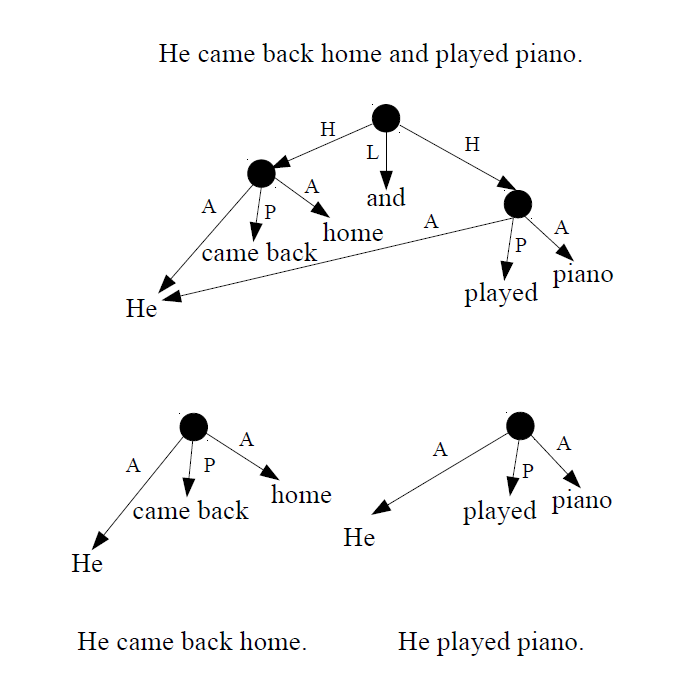
\includegraphics[width=1.2\textwidth,height=48mm]{ucca_simplification}  
    \end{minipage}
}
\end{frame}

\begin{frame}
\frametitle{UCCA Data}
\begin{itemize}
 \item English Wikipedia articles (Wiki).
 \item English-French-German parallel corpus from \\ \textit{Twenty Thousand Leagues Under the Sea} (20K).
 \item Reviews from the English Web Treebank (EWT).
\end{itemize}

\vfill
\begin{center}
  \begin{minipage}{.3\textwidth}
\includegraphics[width=\textwidth]{wikipedia.png}\end{minipage}
  \begin{minipage}{.3\textwidth}
\includegraphics[width=\textwidth]{squid.jpg}\end{minipage}
  
  
\includegraphics[width=.3\textwidth]{five-stars.png}
\end{center}
\end{frame}



\section{Transition-based UCCA Parser}

\begin{frame}
\frametitle{TUPA: Transition-based UCCA Parser}

Parses text $w_1 \ldots w_n$ to graph $G$ incrementally by applying transitions to the parser state,
consisting of: stack, buffer and constructed graph.

\pause
\vfill
Initial state:
\scalebox{.9}{
\begin{tikzpicture}[xscale=1.4,every node/.append style={font=\rmfamily,
                    anchor=west,text height=.6ex,text depth=0}, circle]
    \draw[xstep=1,ystep=.5,color=gray] (-.01,0) grid (1,.5);
    \node[style={font=\sffamily}] at (-.1,.8) {stack};
    \node[fill=black] at (.3,.25) {};
    \draw[xstep=1,ystep=.5,color=gray] (2,0) grid (9,.5);
    \node[style={font=\sffamily}] at (8,.8) {buffer};
    \node at (2,.2) {\small They};
    \node at (3,.2) {\small thought};
    \node at (4,.2) {\small about};
    \node at (5,.2) {\small taking};
    \node at (6,.2) {\small a};
    \node at (7,.2) {\small short};
    \node at (8,.2) {\small break};
\end{tikzpicture}}

\vfill
\pause
\parser{} transitions:

\{\textsc{Shift, Reduce, {\color{blue}Node$_X$}, Left-Edge$_X$, Right-Edge$_X$,}\\
\hspace{5mm}\textsc{{\color{orange}Left-Remote$_X$}, {\color{orange}Right-Remote$_X$}, {\color{red}Swap}, Finish}\}
\end{frame}

\begin{frame}
\frametitle{Training}
An \textit{oracle} provides the transition sequence given the correct graph:

\vfill
\centering
\scalebox{.8}{
\begin{tikzpicture}[level distance=15mm, sibling distance=2cm, ->, thick,
    every node/.append style={font=\rmfamily},
    edge from parent/.append style={nodes={font=\scriptsize}},
    edge from parent path={(\tikzparentnode.center) -- (\tikzchildnode.north)}]
    \node(ROOT)[fill=black, circle] at (3,0) {}
      child {node (They) {They} edge from parent node [left] {A}}
      child {node (thought) {thought} edge from parent node [left] {P}}
      child {node (abouttakingashortbreak) [fill=blue, circle] {} 
      { 
        child {node (to) {about} edge from parent node [right] {R}}
        child {node (takingabreak) [fill=red, circle] {}
        {
          child {node (take) {taking} edge from parent node [above] {F}}      
          child {node (a) {a} edge from parent node [right] {F}} 
          child {node (short) {short} edge from parent [draw=none]}
          child {node (break) {break} edge from parent node [above] {C}}  
        } edge from parent [draw=none]}
      } edge from parent [draw=none]}
      ;
    \draw(abouttakingashortbreak) to node [left] {\scriptsize P} (takingabreak); 
    \draw(ROOT) to node [left] {\scriptsize A} (abouttakingashortbreak);
    \draw[bend left,dashed] (abouttakingashortbreak) to node [auto] {\scriptsize A} (They);
    \draw[bend left] (abouttakingashortbreak) to node [auto] {\scriptsize D} (short);
\end{tikzpicture}}
\[\Downarrow\]
\begin{flushleft}
\footnotesize
\textsc{Shift}, \textsc{Right-Edge$_A$}, \textsc{Shift}, \textsc{Swap}, \textsc{Right-Edge$_P$}, \textsc{Reduce}, \textsc{Shift}, \textsc{Shift}, \textsc{Node$_R$}, \textsc{Reduce}, \textsc{Left-Remote$_A$}, \textsc{Shift}, \textsc{Shift}, \textsc{Node$_C$}, \textsc{Reduce}, \textsc{Shift}, \textsc{Right-Edge$_P$}, \textsc{Shift}, \textsc{Right-Edge$_F$}, \textsc{Reduce}, \textsc{Shift}, \textsc{Swap}, \textsc{Right-Edge$_D$}, \textsc{Reduce}, \textsc{Swap}, \textsc{Right-Edge$_A$}, \textsc{Reduce}, \textsc{Reduce}, \textsc{Shift}, \textsc{Reduce}, \textsc{Shift}, \textsc{Right-Edge$_C$}, \textsc{Finish}
\end{flushleft}
\end{frame}

\begin{frame}
\frametitle{\parser{} Model}
Learns to greedily predict transition based on current state.

\centering
\fbox{\scalebox{.65}{
\begin{minipage}{.6\textwidth}
\begin{tikzpicture}[xscale=1.3,every node/.append style={font=\rmfamily}]
    \node[anchor=west,style={font=\sffamily}] at (-1,.25){stack};
    \draw[xstep=1,ystep=.5,color=gray] (-.01,0) grid (4,.5);
    \node[fill=black, circle] at (.5,.25) {};
    \node[fill=blue, circle] at (2.5,.25) {};
    \node[anchor=west] at (1,.25) {\small They};
    \node[anchor=west] at (3,.25) {\small taking};
\end{tikzpicture}

\vspace{1cm}
\begin{tikzpicture}[xscale=1.3,every node/.append style={font=\rmfamily}]
    \node[anchor=west,style={font=\sffamily}] at (-1,.25){buffer};
    \draw[xstep=1,ystep=.5,color=gray] (-.01,0) grid (4,.5);
    \node[fill=red, circle] at (.5,.25) {};
    \node[anchor=west] at (1,.25) {\small a};
    \node[anchor=west] at (2,.25) {\small short};
    \node[anchor=west] at (3,.25) {\small break};
\end{tikzpicture}
\end{minipage}
\begin{minipage}{.4\textwidth}
\scalebox{.65}{
\begin{tikzpicture}[xscale=1.5,level distance=1cm, sibling distance=12mm, ->,
    every node/.append style={font=\rmfamily,
                    anchor=west,text height=.6ex,text depth=0},
    edge from parent/.append style={nodes={font=\scriptsize}},
    edge from parent path={(\tikzparentnode.center) -- (\tikzchildnode.north)}]
    \node[anchor=west,style={font=\sffamily}] at (3,0) {graph};
    \draw[color=gray] (.2,.3) rectangle (3.9,-3.2);
    \node(ROOT)[fill=black, circle] at (1.2,0) {}
      child {node (They) {They} edge from parent node [left] {A}}
      child {node {thought} edge from parent node [left] {P}}
      child {node (abouttakingashortbreak) [fill=blue, circle] {}
      {
        child {node {about} edge from parent node [left] {R}}
        child {node (takingabreak) [fill=red, circle] {}
        {
          child {node {taking} edge from parent node [above] {F}}
          child [opacity=0] {node {a} edge from parent node [right] {F}}
          child [opacity=0] {node (short) {short} edge from parent [draw=none]}
          child [opacity=0] {node {break} edge from parent node [right] {C}}
        } edge from parent [draw=none]}
      } edge from parent [draw=none]}
      ;
\end{tikzpicture}
}
\end{minipage}
}}

\scalebox{.65}{
\begin{tikzpicture}[->,every node/.append style={anchor=north,text height=2ex,text depth=0}]
    \tiny
    \tikzstyle{main}=[circle, minimum size=7mm, draw=black!80, node distance=12mm]
    \foreach \i/\word in {1/{They},3/{thought},5/{about},7/{taking},9/{a},11/{short},13/{break}} {
        \node (x\i) at (\i,-1.3) {\Large\textrm\word};
        \node[main, fill=white!100] (h\i) at (\i,0) {LSTM};
        \path (x\i) edge (h\i);
        \node[main, fill=white!100] (i\i) at (\i.5,.8) {LSTM};
        \path (x\i) edge [bend right] (i\i);
        \node[main, fill=white!100] (l\i) at (\i.5,2.3) {LSTM};
        \path (h\i) edge [bend left] (l\i);
        \path (i\i) edge (l\i);
        \node[main, fill=white!100] (k\i) at (\i,3.1) {LSTM};
        \path (i\i) edge [bend left] (k\i);
        \path (h\i) edge [bend left] (k\i);
    }
    \foreach \current/\next in {1/3,3/5,5/7,7/9,9/11,11/13} {
        \path (h\current) edge (h\next);
        \path (i\next) edge (i\current);
        \path (l\current) edge (l\next);
        \path (k\next) edge (k\current);
    }
    \node[main, fill=white!100] (mlp) at (7,4.6) {MLP};
    \foreach \i in {1,5,7,9} {
        \path (l\i) edge (mlp);
        \path (k\i) edge (mlp);
    }
    \coordinate (state) at (10.5,6.5);
    \path (state) edge [bend left] (mlp);
    \node (transition) at (7,5.8) {\large\textsc{Node}$_C$};
    \path (mlp) edge (transition);
\end{tikzpicture}
}
\end{frame}


\section{Cross-lingual Parsing}

\begin{frame}
\frametitle{Shared Task}
\Large
\begin{itemize}
\item Data: English Wiki, English-French-German 20K
     \begin{center}
      \begin{tabular}{lcc}
      & sentences & tokens \\
          \hline
          English-Wiki & 5,142      & 158,573 \\
          English-20K  & 492       & 12,574  \\
          French-20K   & 492       & 12,954  \\
          German-20K   & 6,514      & 144,531
      \end{tabular}
      \end{center}
\item Tracks:
        \begin{itemize}
            \item 
                English $\{$in-domain/out-of-domain$\} \times 
                \{$open/closed$\}$
            \item
                German in-domain $\{$open/closed$\}$
            \item
                French \textit{low-resource} (only 15 training sentences)
        \end{itemize}
\item Baseline: TUPA
\item Evaluation period: January 10--31, 2019
\end{itemize}
\end{frame}

\begin{frame}
\frametitle{Participating Systems}
 8 groups in total:
 \begin{itemize}
 \item
 {\it ​MaskParse@Deski\~{n}}  {\small Orange Labs, Aix-Marseille University}
 \item
 {\it HLT@SUDA} { \small  Soochow University}
 \item
 {\it T\"{u}Pa} {\small   University of T\"{u}bingen}
 \item
 {\it UC Davis} {\small   University of California, Davis}
 \item    
 {\it GCN-Sem}  {\small   University of Wolverhampton}
 \item
    {\it CUNY-PekingU} {\small 	 City University of New York, Peking University}
 \item
{\it DANGNT@UIT.VNU-HCM} {\small   University of Information Technology VNU-HCM}
 \item
{\it XLangMo} {\small  Zhejiang University}
\end{itemize}

\end{frame}

\begin{frame}
    \begin{figure}
        \centering
        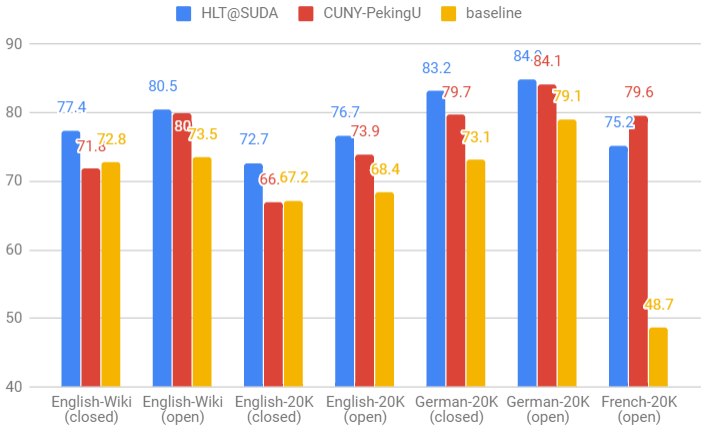
\includegraphics[width=\textwidth]{Capture}
    \end{figure}
\end{frame}



\begin{frame}
\frametitle{Main Findings}

\begin{itemize}
    \item
        HLT@SUDA won 6/7 tracks: \\
        Neural constituency parser + multi-task + BERT \\
        French: trained on all languages, with language embedding
    \pause\item
        CUNY-PekingU won the French (open) track: \\
        TUPA ensemble + synthetic data by machine translation
\end{itemize}
        \pause\vfill
        Surprisingly, results in French were close to English and German
    \begin{itemize}
        \item 
            Demonstrates viability of cross-lingual UCCA parsing
        \item
            Is this because of UCCA's stability in translation?
    \end{itemize}    
\end{frame}


\section{Cross-framework Parsing}


\begin{frame}
    \frametitle{Meaning Representations}

      \begin{flushright}
        \scalebox{.6}{
\begin{tikzpicture}[level distance=2cm, sibling distance=25mm, ->, draw=Indigo, thick, alt=<3->{opacity=.3}{}]
    \node[font=\bf\sffamily\Huge,Indigo] at (-3,0) {UCCA};
    \node (ROOT) [fill=Indigo, circle] {}
      child {node (After) {After} edge from parent node[left] {L\;}}
      child {node (graduation) [fill=Indigo, circle] {}
      {
        child {node {graduation} edge from parent node[left] {P}}
      } edge from parent node[left] {H} }
      child {node {,} edge from parent node[right] {U}}
      child {node (moved) [fill=Indigo, circle] {}
      {
        child {node (Daniel) {Daniel} edge from parent node[left] {A}}
        child {node {moved} edge from parent node[left] {P}}
        child {node [fill=Indigo, circle] {}
        {
          child {node {to} edge from parent node[left] {R}}
          child {node {Copenhagen} edge from parent node[left] {C}}
        } edge from parent node[left] {A} }
      } edge from parent node[right] {H} }
      ;
    \draw[dashed,->] (graduation) to node [auto] {\scriptsize A} (Daniel);
\end{tikzpicture}
        }
      \end{flushright}
    
    \vspace{-23mm}
    
    \scalebox{.6}{
\begin{tikzpicture}[alt=<2>{opacity=.3}{},alt=<4->{opacity=.3}{}, thick]
\node[font=\bf\sffamily\Huge,DarkGreen] at (0,6) {AMR};
\graph[layered layout, sibling distance=4cm, layer distance=2cm, nodes={ellipse,draw=DarkGreen}, edges={nodes={sloped}, DarkGreen}]{
a4 Copenhagen[as={Copenhagen}];
a2 Daniel[as={Daniel}];
a1[as={person}];
a0[as={move-01}];
a3[as={city}];
a2[as={name}];
a5[as={after}];
a4[as={name}];
a6[as={graduate-01}];

a1 ->  ["name"' above] a2;
a0 ->  ["ARG0"' above] a1;
a0 ->  ["ARG2"' above] a3;
a0 ->  ["time"' above] a5;
a3 ->  ["name"' above] a4;
a2 ->  ["op1"' above] a2 Daniel;
a5 ->  ["op1"' above] a6;
a4 ->  ["op1"' above] a4 Copenhagen;
};
\draw[->, above, DarkGreen] (a6) to node[sloped] {ARG0} (a1);
\end{tikzpicture}
      }
    \vspace{-15mm}
    
    \begin{flushright}
    \begin{minipage}{.01\textwidth}
      \begin{tikzpicture}[alt=<2-3>{opacity=.3}{}]
        \node[font=\bf\sffamily\Large,DarkRed] {DM};
      \end{tikzpicture}
    \end{minipage}
    \begin{minipage}{.6\textwidth}
        \rmfamily
        \scalebox{.7}{
\begin{dependency}[theme=simple,edge style={-{Latex[length=2mm]}, color=DarkRed}, alt=<2-3>{opacity=.3}{},
            text only label, label style={above, color=DarkRed, font=\bf\ttfamily}, font=\small, thick]
    \begin{deptext}[column sep=1em,ampersand replacement=\^]
	After \^ graduation \^ , \^ Daniel \^ moved \^ to \^ Copenhagen \\
    \end{deptext}
    \deproot{5}{top}
    \depedge{1}{2}{ARG2}
    \depedge{1}{5}{ARG1}
    \depedge{5}{4}{ARG1}
    \depedge{6}{5}{ARG1}
    \depedge{6}{7}{ARG2}
\end{dependency}
    }
    \end{minipage}
    \end{flushright}
\end{frame}


\begin{frame}
\frametitle{Syntactic Representations}
    {\color{DarkBlue}\bf\sffamily\Large UD} (Universal Dependencies)
    
    \begin{center}
    \rmfamily
    \begin{dependency}[text only label, edge style={-{Latex[length=2mm]}, color=DarkBlue}, thick,
                       label style={above, color=DarkBlue, font=\bf\ttfamily}, font=\small]
    \begin{deptext}[column sep=.8em,ampersand replacement=\^]
    After \^ graduation \^ , \^ Daniel \^ moved \^ to \^ Copenhagen \\
    \end{deptext}
        \depedge{2}{1}{case}
        \depedge{2}{3}{punct}
        \depedge{5}{4}{nsubj}
        \depedge[edge end x offset=-2pt]{5}{2}{obl}
        \depedge{7}{6}{case}
        \deproot[edge unit distance=2.5ex]{5}{root}
        \depedge{5}{7}{obl}
    \end{dependency}
    \end{center}
\end{frame}


\begin{frame}
    \frametitle{Data}
    \fbox{UCCA training data is scarce}
    \begin{center}
    \begin{minipage}{.15\textwidth}
      (English)
    \end{minipage}
    \begin{minipage}{.7\textwidth}
    \pgfplotstableread[row sep=\\,col sep=&]{
    	corpus & total \\
        \color{DarkBlue} UD & 17062 \\
        \color{DarkRed} \textbf{DM} & 33964 \\
        \color{DarkGreen} AMR & 36521 \\
        \color{Indigo} \textbf{UCCA} & 5141 \\
        }\english
        \begin{tikzpicture}
        \begin{axis}[
        xbar stacked,
        width=10cm,
        height=39mm,
        xmin=0,
        xmax=60000,
        xtick=\empty,
        ytick=data,
        yticklabels from table={\english}{corpus},
        axis x line=none,
        ]
        \addplot [fill=Navy, point meta=explicit symbolic,
        nodes near coords={\pgfmathprintnumber\pgfplotspointmeta~sentences},
        nodes near coords align={anchor=west}] table [x=total,y expr=\coordindex,meta=total] {\english};
        \end{axis}
        \end{tikzpicture}
    \end{minipage}
    \end{center}
    
    \pause
    \vfill
    
    \begin{flushright}
        \fbox{and domains are limited.}
    \end{flushright}
    \begin{center}
    \begin{tabular}{llll}
        \color{Indigo} \textbf{UCCA}  & \color{DarkGreen} AMR  & \color{DarkRed} \textbf{DM}  & \color{NavyBlue} UD  \\
    	Wikipedia & blogs & news & blogs \\ books & news && news \\ & emails && emails \\ & reviews && reviews \\ &&& Q\&A
    \end{tabular}
    \end{center}
\end{frame}

\def\convertedudgraduation{
  \begin{tikzpicture}[level distance=15mm, ->, draw=DarkBlue, thick,
      every node/.append style={sloped,anchor=south,auto=false,font=\scriptsize},
      level 1/.style={sibling distance=16mm},
      level 2/.style={sibling distance=13mm},
      edge from parent path={(\tikzparentnode.center) -- (\tikzchildnode.north)}]
    \tikzstyle{word} = [font=\rmfamily,color=black]
    \node (ROOT) [fill=DarkBlue,circle] {}
      child {node (after) [fill=DarkBlue,circle] {}
      {
        child {node [word] {After{\color{white}g}\quad\quad} edge from parent node {case}}
        child {node [word] {\quad graduation\quad\quad} edge from parent node {head}}
      } edge from parent node {obl}}
      child {node {}
      {
        child {node [word] (comma) {\quad,{\color{white}g}} edge from parent [draw=none]}
      } edge from parent [draw=none]}
      child {node {}
      {
        child {node [word] (Daniel) {Daniel{\color{white}g}} edge from parent [draw=none]}
      } edge from parent [draw=none]}
      child {node {}
      {
        child {node [word] (moved) {moved{\color{white}g}} edge from parent [draw=none]}
      } edge from parent [draw=none]}
      child {node (to) [fill=DarkBlue,circle] {}
      {
          child {node [word] {to{\color{white}g}} edge from parent node {case}}
          child {node [word] {Copenhagen{\color{white}g}} edge from parent node {head}}
      } edge from parent node {obl}}
      ;
      \draw (ROOT) to node {punct} (comma);
      \draw (ROOT) to node {nsubj} (Daniel);
      \draw (ROOT) to node {head} (moved);
  \end{tikzpicture}
}


\begin{frame}
\frametitle{Conversion}

\begin{minipage}{.04\textwidth}
\vspace{4mm}
\color{DarkGreen} AMR\\
\vspace{13mm}
\color{DarkRed} DM\\
\vspace{14mm}
\color{DarkBlue} UD
\end{minipage}
\begin{minipage}{.45\textwidth}
  \centering
  \scalebox{.6}{
  \begin{tikzpicture}[->,draw=DarkGreen,
      every node/.append style={sloped,anchor=south,auto=false,font=\tiny},
      level 1/.style={level distance=14mm,sibling distance=26mm},
      level 2/.style={level distance=13mm},
      level 3/.style={level distance=12mm}]
    \node (ROOT) [draw=DarkGreen,ellipse] {move-01}
      child {node [draw=DarkGreen,ellipse] {city}
      {
        child {node [draw=DarkGreen,ellipse] {name}
        {
            child {node [draw=DarkGreen,ellipse] {"Copenhagen"} edge from parent node {op1} }
        } edge from parent node {name} }
      } edge from parent node {ARG2} }
      child {node [draw=DarkGreen,ellipse] {after}
      {
            child {node (graduation) [draw=DarkGreen,ellipse] {graduate-01} edge from parent node {op1} }
      } edge from parent node {time} }
      child {node (Daniel) [draw=DarkGreen,ellipse] {person}
      {
        child {node [draw=DarkGreen,ellipse] {name}
        {
            child {node [draw=DarkGreen,ellipse] {"Daniel"} edge from parent node {op1} }
        } edge from parent node {name} }
      } edge from parent node {ARG0} }
      ;
      \draw (graduation) to node {ARG0} (Daniel);
  \end{tikzpicture}
  }
  
  \vspace{5mm}
  \scalebox{.6}{
    \begin{dependency}[theme=simple,text only label, font=\small, edge style={color=DarkRed},
                       label style={above, color=DarkRed, font=\bf\ttfamily}]
    \begin{deptext}[column sep=.8em,ampersand replacement=\^]
    After \^ graduation \^ , \^ Daniel \^ moved \^ to \^ Copenhagen \\
    \end{deptext}
        \depedge{1}{2}{ARG2}
        \depedge{5}{4}{ARG1}
        \depedge[edge end x offset=-2pt]{1}{5}{ARG1}
        \deproot[edge unit distance=3.5ex]{5}{top}
        \depedge[edge start x offset=-1pt, edge end x offset=3pt]{5}{7}{ARG2}
        \depedge[edge end x offset=5pt]{6}{5}{ARG1}
        \depedge{6}{7}{ARG2}
    \end{dependency}
    }
    
  \vspace{5mm}
  \scalebox{.6}{
    \begin{dependency}[text only label, edge style={color=DarkBlue},
                       label style={above, color=DarkBlue, font=\bf\ttfamily}, font=\small]
    \begin{deptext}[column sep=.8em,ampersand replacement=\^]
    After \^ graduation \^ , \^ Daniel \^ moved \^ to \^ Copenhagen \\
    \end{deptext}
        \depedge{2}{1}{case}
        \depedge{2}{3}{punct}
        \depedge{5}{4}{nsubj}
        \depedge[edge end x offset=-2pt]{5}{2}{obl}
        \depedge{7}{6}{case}
        \deproot[edge unit distance=2.5ex]{5}{root}
        \depedge{5}{7}{obl}
    \end{dependency}
    }

\end{minipage}
\begin{minipage}{.02\textwidth}
\vspace{7mm}
\Rightarrow
\vspace{16mm}
\Rightarrow
\vspace{20mm}
\Rightarrow
\end{minipage}
\begin{minipage}{.45\textwidth}

  \centering
  \scalebox{.6}{
  \begin{tikzpicture}[level distance=16mm, ->, draw=DarkGreen, thick,
      every node/.append style={sloped,anchor=south,auto=false,font=\scriptsize},
      level 1/.style={sibling distance=28mm},
      level 2/.style={sibling distance=14mm},
      level 3/.style={sibling distance=12mm}]
    \tikzstyle{word} = [font=\rmfamily,color=black]
    \node (ROOT) [word] {moved}
      child {node [word] {After}
      {
            child {node (graduation) [word] {graduation} edge from parent node {op} }
      } edge from parent node {time} }
      child {node (Daniel) [fill=DarkGreen,circle] {}
      {
        child {node [word] {Daniel} edge from parent node {name} }
      } edge from parent node {ARG0} }
      child {node [fill=DarkGreen,circle] {}
      {
        child {node [word] {Copenhagen} edge from parent node {name} }
      } edge from parent node {ARG2} }
      ;
      \draw[dashed] (graduation) to node {ARG0} (Daniel);
  \end{tikzpicture}}

  \vspace{5mm}
  \scalebox{.6}{
  \begin{tikzpicture}[level distance=14mm, ->, draw=DarkRed, thick,
      every node/.append style={sloped,anchor=south,auto=false,font=\scriptsize},
      level 1/.style={sibling distance=29mm,level distance=6mm},
      level 2/.style={sibling distance=16mm,level distance=14mm},
      edge from parent path={(\tikzparentnode.center) -- (\tikzchildnode.north)}]
    \tikzstyle{word} = [font=\rmfamily,color=black]
    \node (ROOT) [fill=DarkRed,circle] {}
      child {node (after) [fill=DarkRed,circle] {}
      {
        child {node [draw=none] {}
        {
          child {node [word] (after_word) {After{\color{white}g}} edge from parent [draw=none]}
        } edge from parent [draw=none] }
        child {node [draw=none] {}
        {
          child {node [word] (graduation) {graduation ,} edge from parent [draw=none]}
        } edge from parent [draw=none] }
      } edge from parent node {root}}
      child {node [draw=none] {}
      {
        child {node (moved) [fill=DarkRed,circle] {}
        {
          child {node [word] {\quad{\color{white}g} Daniel} edge from parent node {ARG1}}
          child {node [word] {moved{\color{white}g}} edge from parent node {head}}
        } edge from parent [draw=none] }
      } edge from parent [draw=none] }
      child {node (to) [fill=DarkRed,circle] {}
      {
        child {node [draw=none] {}
        {
            child {node [word] (to_word) {to{\color{white}g}} edge from parent [draw=none]}
          } edge from parent [draw=none] }
          child {node [draw=none] {}
        {
          child {node [word] (Copenhagen) {Copenhagen{\color{white}g}} edge from parent [draw=none]}
        } edge from parent [draw=none] }
      } edge from parent node {root}}
      ;
      \draw (ROOT) to node {top} (moved);
      \draw (after) to node {head} (after_word);
      \draw (after) to node {ARG2} (graduation);
      \draw[dashed] (after) to node {ARG1} (moved);
      \draw[dashed] (to) to node {ARG1} (moved);
      \draw (to) to node {head} (to_word);
      \draw (moved) to node {ARG2} (Copenhagen);
      \draw[dashed] (to) to node {ARG2} (Copenhagen);
  \end{tikzpicture}}

  \vspace{5mm}
  \scalebox{.6}{\convertedudgraduation}
\end{minipage}
\end{frame}


\begin{frame}
    \frametitle{Multi-task}
    \begin{minipage}{.05\pagewidth}
    \scalebox{6}{\{}
    \end{minipage}
    \begin{minipage}{.3\pagewidth}
        \scalebox{.3}{
\begin{tikzpicture}[level distance=2cm, sibling distance=25mm, ->, draw=Indigo, thick,
    edge from parent/.append style={nodes={font=\scriptsize}},
    edge from parent path={(\tikzparentnode.center) -- (\tikzchildnode.north)}]
    \node (ROOT) [fill=Indigo, circle] {}
      child {node (After) {After} edge from parent node[left] {L\;}}
      child {node (graduation) [fill=Indigo, circle] {}
      {
        child {node {graduation} edge from parent node[left] {P}}
      } edge from parent node[left] {H} }
      child {node {,} edge from parent node[right] {U}}
      child {node (moved) [fill=Indigo, circle] {}
      {
        child {node (Daniel) {Daniel} edge from parent node[left] {A}}
        child {node {moved} edge from parent node[left] {P}}
        child {node [fill=Indigo, circle] {}
        {
          child {node {to} edge from parent node[left] {R}}
          child {node {Copenhagen} edge from parent node[left] {C}}
        } edge from parent node[left] {A} }
      } edge from parent node[right] {H} }
      ;
    \draw[dashed,->] (graduation) to node [auto] {\scriptsize A} (Daniel);
\end{tikzpicture}
        }
    \end{minipage}
    \begin{minipage}{.24\pagewidth}
    \scalebox{.3}{
\begin{tikzpicture}
\graph[layered layout, sibling distance=4cm, layer distance=2cm, nodes={ellipse,draw=DarkGreen}, edges={nodes={sloped}, DarkGreen}]{
a4 Copenhagen[as={Copenhagen}];
a2 Daniel[as={Daniel}];
a1[as={person}];
a0[as={move-01}];
a3[as={city}];
a2[as={name}];
a5[as={after}];
a4[as={name}];
a6[as={graduate-01}];

a1 ->  ["name"' above] a2;
a0 ->  ["ARG0"' above] a1;
a0 ->  ["ARG2"' above] a3;
a0 ->  ["time"' above] a5;
a3 ->  ["name"' above] a4;
a2 ->  ["op1"' above] a2 Daniel;
a5 ->  ["op1"' above] a6;
a4 ->  ["op1"' above] a4 Copenhagen;
};
\draw[->, above, DarkGreen] (a6) to node[sloped] {ARG0} (a1);
\end{tikzpicture}
      }
    \end{minipage}
    \begin{minipage}{.21\pagewidth}
        \rmfamily
        \scalebox{.3}{
\begin{dependency}[theme=simple,edge style={-{Latex[length=2mm]}, color=DarkRed},
            text only label, label style={above, color=DarkRed, font=\bf\ttfamily}, font=\small]
    \begin{deptext}[column sep=1.5em,ampersand replacement=\^]
	After \^ graduation \^ , \^ Daniel \^ moved \^ to \^ Copenhagen \\
    \end{deptext}
    \deproot{5}{top}
    \depedge{1}{2}{ARG2}
    \depedge{1}{5}{ARG1}
    \depedge{5}{4}{ARG1}
    \depedge{6}{5}{ARG1}
    \depedge{6}{7}{ARG2}
\end{dependency}
    }
    
        \scalebox{.3}{
    \begin{dependency}[edge style={-{Latex[length=2mm]}, color=DarkBlue},
        text only label, label style={above, color=DarkBlue, font=\bf\ttfamily}, font=\small]
    \begin{deptext}[column sep=1.5em,ampersand replacement=\^, color=DarkBlue]
    After \^ graduation \^ , \^ Daniel \^ moved \^ to \^ Copenhagen \\
    \end{deptext}
        \depedge[edge unit distance=1em]{2}{1}{case}
        \depedge[edge unit distance=1em]{2}{3}{punct}
        \depedge[edge unit distance=1em, edge start x offset=-4mm]{5}{4}{nsubj}
        \depedge[edge unit distance=1em, edge end x offset=-3mm]{5}{2}{obl}
        \depedge[edge unit distance=1em]{7}{6}{case}
        \deproot[edge unit distance=1em]{5}{root}
        \depedge[edge unit distance=1.5em, edge start x offset=1mm]{5}{7}{obl}
    \end{dependency}
    }
    \end{minipage}
    \begin{minipage}{.05\pagewidth}
    \scalebox{6}{\}}
    \end{minipage}
    
    \pause
    
    \vfill
    
    Multi-task TUPA model:
    
    \vspace{-7mm}
    
    \begin{center}\scalebox{.3}{\Huge
       \begin{tikzpicture}[-{Latex[length=3mm]},very thick]
       \tikzstyle{main}=[rounded rectangle, minimum size=35mm, draw=black!80, node distance=12mm]
       \node[main] (specific) at (0,12) {Task-specific BiLSTM};
       \node[main,color=DarkCyan] (shared) at (22,12) {Shared BiLSTM};
       \foreach \i/\word in {-4/{After},4/{graduation},17/{to},25/{Copenhagen}} {
           \node (x\i) at (\i,3) {\word};
           \node[main, minimum size=16mm, fill=DarkCyan, draw=none] (e\i) at (\i,6) {};
           \path[color=DarkCyan] (x\i) edge (e\i);
           \path (e\i) edge (specific);
           \path[color=DarkCyan] (e\i) edge (shared);
       }
        \node (x4) at (10.5,3) {\ldots};
        \node[main] (mlp) at (10.5,15) {MLP};
        \path (specific) edge (mlp);
        \path[color=DarkCyan] (shared) edge (mlp);
        \node (transition) at (10.5,17.8) {};
        \path (mlp) edge node[right] {} (transition);
       \end{tikzpicture}}
    \end{center}
\end{frame}

\begin{frame}
\frametitle{Results}

\pgfplotstableread[row sep=\\,col sep=&]{
	aux & pf1 & rf1 \\
	+All & 74.4 & 52 \\
	+{\color{DarkRed} DM} + {\color{NavyBlue} UD} & 74.9 & 51.2 \\
	+{\color{DarkGreen} AMR} + {\color{NavyBlue} UD} & 73.8 & 48.5 \\
	+{\color{DarkGreen} AMR} + {\color{DarkRed} DM} & 74.7 & 51.4 \\
	+\color{NavyBlue} UD & 74.1 & 50.8 \\
	+\color{DarkRed} DM & 74.8 & 53.9 \\
	+\color{DarkGreen} AMR & 73.7 & 49.9 \\
	Single & 73.6 & 51.5 \\
}\indomaindata

\pgfplotstableread[row sep=\\,col sep=&]{
	aux & pf1 & rf1 \\
	+All & 71 & 29.6 \\
	+{\color{DarkRed} DM} + {\color{NavyBlue} UD} & 70.6 & 28.4 \\
	+{\color{DarkGreen} AMR} + {\color{NavyBlue} UD} & 70 & 29.4 \\
	+{\color{DarkGreen} AMR} + {\color{DarkRed} DM} & 70.5 & 27.3 \\
	+\color{NavyBlue} UD & 69.7 & 28.7 \\
	+\color{DarkRed} DM & 70.7 & 25.9 \\
	+\color{DarkGreen} AMR & 69.5 & 27.5 \\
	Single & 69 & 26.7 \\
}\outdomaindata

\pgfplotstableread[row sep=\\,col sep=&]{
	aux & pf1 & rf1 \\
	+\color{NavyBlue} UD & 70.1 & 20.3 \\
	Single & 67.6 & 13.9 \\
}\frenchdata

\pgfplotstableread[row sep=\\,col sep=&]{
	aux & pf1 & rf1 \\
	+\color{NavyBlue} UD & 73.2 & 35.5 \\
	Single & 72.5 & 27.1 \\
}\germandata

\begin{center}
    \small
	\begin{minipage}{.4\textwidth}
	\begin{tikzpicture}
		    \begin{axis}[
		    xbar,
		    width=.7\textwidth,
		    height=.91\textheight,
		    xmin=65,
		    xmax=80,
		    bar width=3mm,
		    xtick=\empty,
		    ytick=data,
		    yticklabels from table={\indomaindata}{aux},
		    axis x line=none,
		    axis line style={draw=none},
		    clip=false,
		    title={English (in-domain)}
		    ]
%		    \addplot [fill=Crimson, point meta=explicit symbolic,nodes near coords,
%		    nodes near coords align={anchor=west}] table [x=rf1,y expr=\coordindex,meta=rf1] {\indomaindata};
		    \addplot [fill=Navy, point meta=explicit symbolic,nodes near coords,
		    nodes near coords align={anchor=west}] table [x=pf1,y expr=\coordindex,meta=pf1] {\indomaindata};
		    \end{axis}
	\end{tikzpicture}
	\end{minipage}
	\hfill
	\begin{minipage}{.23\textwidth}
	\vspace{-3.5mm}
	\begin{tikzpicture}
		    \begin{axis}[
		    xbar,
		    width=1.7\textwidth,
		    height=.9\textheight,
		    xmin=65,
		    xmax=80,
		    bar width=3mm,
		    xtick=\empty,
		    axis x line=none,
		    axis y line=none,
		    clip=false,
		    title={English (ood)}
		    ]
%		    \addplot [fill=Crimson, point meta=explicit symbolic,nodes near coords,
%		    nodes near coords align={anchor=west}] table [x=rf1,y expr=\coordindex,meta=rf1] {\outdomaindata};
		    \addplot [fill=Navy, point meta=explicit symbolic,nodes near coords,
		    nodes near coords align={anchor=west}] table [x=pf1,y expr=\coordindex,meta=pf1] {\outdomaindata};
		    \end{axis}
	\end{tikzpicture}
	\end{minipage}
	\begin{minipage}{.22\textwidth}
	\begin{tikzpicture}
		    \begin{axis}[
		    xbar,
		    width=1.2\textwidth,
		    height=.3\textheight,
		    xmin=65,
		    xmax=80,
		    bar width=3mm,
		    xtick=\empty,
		    ytick=data,
		    yticklabels from table={\frenchdata}{aux},
		    axis x line=none,
		    axis line style={draw=none},
		    clip=false,
		    title={French (in-domain)}
		    ]
%		    \addplot [fill=Crimson, point meta=explicit symbolic,nodes near coords,
%		    nodes near coords align={anchor=west}] table [x=rf1,y expr=\coordindex,meta=rf1] {\frenchdata};
		    \addplot [fill=Navy, point meta=explicit symbolic,nodes near coords,
		    nodes near coords align={anchor=west}] table [x=pf1,y expr=\coordindex,meta=pf1] {\frenchdata};
		    \end{axis}
	\end{tikzpicture}

    \vspace{1cm}
	
	\begin{tikzpicture}
		    \begin{axis}[
		    xbar,
		    width=1.2\textwidth,
		    height=.3\textheight,
		    xmin=65,
		    xmax=80,
		    bar width=3mm,
		    reverse legend,
	        legend style={at={(axis cs:0,1.5)},anchor=south west},
		    xtick=\empty,
		    ytick=data,
		    yticklabels from table={\germandata}{aux},
		    axis x line=none,
		    axis line style={draw=none},
		    clip=false,
		    title={German (in-domain)}
		    ]
%		    \addplot [fill=Crimson, point meta=explicit symbolic,nodes near coords,
%		    nodes near coords align={anchor=west}] table [x=rf1,y expr=\coordindex,meta=rf1] {\germandata};
		    \addplot [fill=Navy, point meta=explicit symbolic,nodes near coords,
		    nodes near coords align={anchor=west}] table [x=pf1,y expr=\coordindex,meta=pf1] {\germandata};
%		    \legend{remote F1,primary F1}
		    \end{axis}
	\end{tikzpicture}
	\end{minipage}
\end{center}
\end{frame}

\begin{frame}
TUPA output: \\

\scalebox{.7}{
\begin{tikzpicture}[->,level distance=9mm,
  level 1/.style={sibling distance=8cm},
  level 2/.style={sibling distance=35mm},
  level 3/.style={ sibling distance=9mm},
  level 4/.style={ sibling distance=13mm},
  level 5/.style={ sibling distance=8mm},
  every circle node/.append style={fill=black},
  edge from parent path={(\tikzparentnode.center) -- (\tikzchildnode.east)}]
  \tikzstyle{word} = [font=\rmfamily,color=black,rotate=40,anchor=east]
  \node (1_1) [circle] {}
  {
  child {node (1_2) [circle] {}
    {
    child {node (1_5) [circle] {}
      {
      child {node (1_10) [word] {No} edge from parent node[auto] {\scriptsize $E$}}
      child {node (1_11) [word] {transoceanic} edge from parent node[auto] {\scriptsize $E$}}
      child {node (1_12) [word] {navigational} edge from parent node[auto] {\scriptsize $E$}}
      child {node (1_13) [word] {undertaking} edge from parent node[auto] {\scriptsize $C$}} }edge from parent node[auto] {\scriptsize $A$}}
    child {node (1_6) [circle] {}
      {
      child {node (1_14) [word] {has} edge from parent node[auto] {\scriptsize $F$}}
      child {node (1_15) [word] {been} edge from parent node[auto] {\scriptsize $E$}}
      child {node (1_16) [word] {conducted} edge from parent node[auto] {\scriptsize $C$}} }edge from parent node[auto] {\scriptsize $P$}}
    child {node (1_7) [circle] {}
      {
      child {node (1_17) [word] {with} edge from parent node[auto] {\scriptsize $R$}}
      child {node (1_18) [circle] {}
        {
        child {node (1_25) [circle] {}
          {
          child {node (1_28) [word] {more} edge from parent node[auto] {\scriptsize $E$}}
          child {node (1_29) [word] {ability} edge from parent node[auto] {\scriptsize $C$}} }edge from parent node[auto] {\scriptsize $C$}}
        child {node (1_27) [circle] {}
          {
          child {node (1_30) [word] {no} edge from parent node[auto] {\scriptsize $E$}}
          child {node (1_31) [circle] {}
            {
            child {node (1_32) [word] {business} edge from parent node[auto] {\scriptsize $E$}}
            child {node (1_33) [word] {dealings} edge from parent node[auto] {\scriptsize $C$}} }edge from parent node[auto] {\scriptsize $C$}} }edge from parent node[auto] {\scriptsize $C$}} }edge from parent node[auto] {\scriptsize $C$}} }edge from parent node[auto] {\scriptsize $A$}} }edge from parent node[auto] {\scriptsize $H$}}
  child {node (1_3) [circle] {}
    {
    child {node (1_8) [circle] {}
      {
      child {node (1_19) [word] {have} edge from parent node[auto] {\scriptsize $F$}}
      child {node (1_20) [word] {been} edge from parent node[auto] {\scriptsize $E$}}
      child {node (1_21) [word] {crowned} edge from parent node[auto] {\scriptsize $C$}} }edge from parent node[auto] {\scriptsize $P$}}
    child {node (1_9) [circle] {}
      {
      child {node (1_22) [word] {with} edge from parent node[auto] {\scriptsize $R$}}
      child {node (1_23) [word] {greater} edge from parent node[auto] {\scriptsize $D$}}
      child {node (1_24) [word] {success} edge from parent node[auto] {\scriptsize $P$}} }edge from parent node[auto] {\scriptsize $A$}} }edge from parent node[auto] {\scriptsize $H$}} }
;
\end{tikzpicture}}

\vspace{-5mm}

Multi-task TUPA output: \\
(+AMR+DM+UD)

\vspace{-5mm}

\scalebox{.7}{
\begin{tikzpicture}[->,level distance=9mm,
  level 1/.style={sibling distance=8cm},
  level 2/.style={sibling distance=28mm},
  level 3/.style={ sibling distance=9mm},
  every circle node/.append style={fill=black},
  edge from parent path={(\tikzparentnode.center) -- (\tikzchildnode.east)}]
  \tikzstyle{word} = [font=\rmfamily,color=black,rotate=40,anchor=east]
  \node (1_1) [circle] {}
  {
  child {node (1_2) [circle] {}
    {
    child {node (1_6) [circle] {}
      {
      child {node (1_12) [word] {No} edge from parent node[auto] {\scriptsize $E$}}
      child {node (1_13) [word] {transoceanic} edge from parent node[auto] {\scriptsize $E$}}
      child {node (1_14) [word] {navigational} edge from parent node[auto] {\scriptsize $E$}}
      child {node (1_15) [word] {undertaking} edge from parent node[auto] {\scriptsize $C$}} }edge from parent node[auto] {\scriptsize $A$}}
    child {node (1_7) [circle] {}
      {
      child {node (1_16) [word] {has} edge from parent node[auto] {\scriptsize $F$}}
      child {node (1_17) [word] {been} edge from parent node[auto] {\scriptsize $F$}}
      child {node (1_18) [word] {conducted} edge from parent node[auto] {\scriptsize $C$}} }edge from parent node[auto] {\scriptsize $P$}}
    child {node (1_8) [circle] {}
      {
      child {node (1_19) [word] {with} edge from parent node[auto] {\scriptsize $R$}}
      child {node (1_20) [word] {more} edge from parent node[auto] {\scriptsize $E$}}
      child {node (1_21) [word] {ability} edge from parent node[auto] {\scriptsize $C$}} }edge from parent node[auto] {\scriptsize $A$}} }edge from parent node[auto] {\scriptsize $H$}}
  child {node (1_4) [circle] {}
    {
    child {node (1_9) [circle] {}
      {
      child {node (1_22) [word] {no} edge from parent node[auto] {\scriptsize $E$}}
      child {node (1_23) [word] {business} edge from parent node[auto] {\scriptsize $E$}}
      child {node (1_24) [word] {dealings} edge from parent node[auto] {\scriptsize $C$}} }edge from parent node[auto] {\scriptsize $A$}}
    child {node (1_10) [circle] {}
      {
      child {node (1_25) [word] {have} edge from parent node[auto] {\scriptsize $F$}}
      child {node (1_26) [word] {been} edge from parent node[auto] {\scriptsize $F$}}
      child {node (1_27) [word] {crowned} edge from parent node[auto] {\scriptsize $C$}} }edge from parent node[auto] {\scriptsize $P$}}
    child {node (1_11) [circle] {}
      {
      child {node (1_28) [word] {with} edge from parent node[auto] {\scriptsize $R$}}
      child {node (1_29) [word] {greater} edge from parent node[auto] {\scriptsize $E$}}
      child {node (1_30) [word] {success} edge from parent node[auto] {\scriptsize $C$}} }edge from parent node[auto] {\scriptsize $A$}} }edge from parent node[auto] {\scriptsize $H$}} }
;
\end{tikzpicture}}
\end{frame}



\section{What Distinguishes Meaning Representations?}


\begin{frame}
\frametitle{UCCA vs. UD}
    \begin{minipage}[t]{.17\textwidth}
      \onslide<2->{
        \fbox{Many formal differences.}
      }
    \end{minipage}
    \begin{minipage}{.5\textwidth}
        \scalebox{.77}{
\begin{tikzpicture}[level distance=2cm, sibling distance=25mm, ->, draw=Indigo, thick]
    \node[anchor=west,font=\Large] at (-3,.5) {Semantic representation:};
    \node[anchor=west,font=\bf\sffamily\LARGE,Indigo] at (-3,0) {UCCA};
    \node (ROOT) [fill=Indigo, circle] {}
      child {node (After) {After} edge from parent node[left] {L\;}}
      child {node (graduation) [fill=Indigo, circle] {}
      {
        child {node {graduation} edge from parent node[left] {P}}
      } edge from parent node[left] {H} }
      child {node {,} edge from parent node[right] {U}}
      child {node (moved) [fill=Indigo, circle] {}
      {
        child {node (Daniel) {Daniel} edge from parent node[left] {A}}
        child {node {moved} edge from parent node[left] {P}}
        child {node [fill=Indigo, circle] {}
        {
          child {node {to} edge from parent node[left] {R}}
          child {node {Copenhagen} edge from parent node[left] {C}}
        } edge from parent node[left] {A} }
      } edge from parent node[right] {H} }
      ;
    \draw[dashed,->] (graduation) to node [auto] {\scriptsize A} (Daniel);
\end{tikzpicture}
        }
    \end{minipage}
    \begin{minipage}{.2\textwidth}
      \onslide<3->{
        \fbox{What about \textit{content}?}
        \vspace{4cm}
      }
    \end{minipage}
      
    \vspace{-1cm}
      
    Syntactic representation:
    
    {\color{DarkBlue}\bf\sffamily\Large UD}
    
    \vspace{-4mm}
    
    \rmfamily
    \begin{dependency}[text only label, edge style={-{Latex[length=2mm]}, color=DarkBlue, thick},
                       label style={above, color=DarkBlue, font=\bf\ttfamily}, font=\small]
    \begin{deptext}[column sep=.8em,ampersand replacement=\^]
    After \^ graduation \^ , \^ Daniel \^ moved \^ to \^ Copenhagen \\
    \end{deptext}
        \depedge{2}{1}{case}
        \depedge{2}{3}{punct}
        \depedge{5}{4}{nsubj}
        \depedge[edge end x offset=-2pt]{5}{2}{obl}
        \depedge{7}{6}{case}
        \deproot[edge unit distance=2.5ex]{5}{root}
        \depedge{5}{7}{obl}
    \end{dependency}
\end{frame}


\begin{frame}
\frametitle{Assimilating the Graph Structures}

\begin{minipage}{.04\textwidth}
\color{DarkBlue} UD
\end{minipage}
\only<-2>{
\begin{minipage}{.45\textwidth}
  \centering
  \scalebox{.6}{
    \begin{dependency}[text only label, edge style={color=DarkBlue},
                       label style={above, color=DarkBlue, font=\bf\ttfamily}, font=\small]
    \begin{deptext}[column sep=.8em,ampersand replacement=\^]
    After \^ graduation \^ , \^ Daniel \^ moved \^ to \^ Copenhagen \\
    \end{deptext}
        \depedge{2}{1}{case}
        \depedge{2}{3}{punct}
        \depedge{5}{4}{nsubj}
        \depedge[edge end x offset=-2pt]{5}{2}{obl}
        \depedge{7}{6}{case}
        \deproot[edge unit distance=2.5ex]{5}{root}
        \depedge{5}{7}{obl}
    \end{dependency}
    }
\end{minipage}
\begin{minipage}{.02\textwidth}
\Rightarrow
\end{minipage}
\begin{minipage}{.4\textwidth}
  \centering
  \scalebox{.55}{\convertedudgraduation}
\end{minipage}
}
\only<3->{
\begin{minipage}{.9\textwidth}
  \centering
  \scalebox{.9}{\convertedudgraduation}
\end{minipage}
}

\pause
\vfill

Now we can evaluate by matching edges (UCCA unlabeled evaluation)

\pause
\vfill

\begin{minipage}{.5\textwidth}
\scalebox{.7}{
\begin{tikzpicture}[level distance=17mm, sibling distance=25mm, ->, draw=Indigo, thick]
    \node[anchor=west,font=\sffamily\LARGE,Indigo] at (-4,0) {UCCA};
    \node (ROOT) [fill=Indigo, circle] {}
      child {node (After) {After} edge from parent node[left] {L\;}}
      child {node (graduation) [fill=Indigo, circle] {}
      {
        child {node {graduation} edge from parent node[left] {P}}
      } edge from parent node[left] {H} }
      child {node {,} edge from parent node[right] {U}}
      child {node (moved) [fill=Indigo, circle] {}
      {
        child {node (Daniel) {Daniel} edge from parent node[left] {A}}
        child {node {moved} edge from parent node[left] {P}}
        child {node [fill=Indigo, circle] {}
        {
          child {node {to} edge from parent node[left] {R}}
          child {node {Copenhagen} edge from parent node[left] {C}}
        } edge from parent node[left] {A} }
      } edge from parent node[right] {H} }
      ;
    \draw[dashed,->] (graduation) to node [auto] {\scriptsize A} (Daniel);
\end{tikzpicture}
}
\end{minipage}
\pause
\begin{minipage}[b]{.4\textwidth}
    \large
    \begin{tabular}{c|c|c}
        \textbf{P} & \textbf{R} & \textbf{F1} \\ \hline
        $\frac89=89\%$ & $\frac8{10}=80\%$ & 84\%
    \end{tabular}
    \vspace{1cm}
\end{minipage}
\end{frame}


\begin{frame}
\frametitle{Confusion Matrix}
\centering
\setlength\tabcolsep{1pt}
\def\arraystretch{.5}
\scalebox{.7}{
\begin{tabular}{lRRRRRRRRRRRRRRRR|R}
 &&&&&&&&&&&&&&&&& \multicolumn{1}{|c}{\textsc{No}} \\
 & \multicolumn{1}{c}{\textbf{A}}
 & \multicolumn{1}{c}{\textbf{A\big|P}} & \multicolumn{1}{c}{\textbf{A\big|S}}
 & \multicolumn{1}{c}{\textbf{C}}
 & \multicolumn{1}{c}{\textbf{D}}
 & \multicolumn{1}{c}{\textbf{E}}
 & \multicolumn{1}{c}{\textbf{F}}
 & \multicolumn{1}{c}{\textbf{G}}
 & \multicolumn{1}{c}{\textbf{H}}
 & \multicolumn{1}{c}{\textbf{L}}
 & \multicolumn{1}{c}{\textbf{N}}
 & \multicolumn{1}{c}{\textbf{P}}
 & \multicolumn{1}{c}{\textbf{Q}}
 & \multicolumn{1}{c}{\textbf{R}}
 & \multicolumn{1}{c}{\textbf{S}}
 & \multicolumn{1}{c}{\textbf{T}}
 & \multicolumn{1}{|c}{\textsc{Match}} \\
\texttt{acl} & 58 &  &  & 1 & 4 & 249 & 1 &  & 48 &  &  & 6 &  &  & 1 & 1 & 409 \\
\texttt{advcl} & 14 &  &  & 12 & 2 & 2 &  & 6 & 512 & 4 &  & 11 &  &  &  &  & 423 \\
\texttt{advmod} & 225 &  & 1 & 69 & 1778 & 332 & 27 & 135 & 14 & 258 & 2 & 2 & 15 & 44 & 9 & 368 & 273 \\
\texttt{amod} & 25 &  &  & 134 & 647 & 837 &  & 1 & 28 &  &  & 7 & 130 & 3 & 269 & 25 & 176 \\
\texttt{appos} & 21 &  &  & 39 & 2 & 34 &  &  & 18 &  &  &  &  &  & 8 &  & 33 \\
\texttt{aux} &  &  &  &  & 384 & 2 & 1335 &  &  & 2 &  & 1 &  & 1 &  &  & 17 \\
\texttt{case} & 11 &  &  & 31 & 27 & 25 & 123 &  &  & 213 & 26 & 11 & 1 & 2629 & 154 & 1 & 262 \\
\texttt{cc} &  &  &  & 8 & 4 & 1 & 4 & 1 & 1 & 1567 & 381 &  & 6 & 12 &  &  & 52 \\
\texttt{ccomp} & 345 &  &  & 1 &  & 1 &  &  & 36 &  &  & 2 &  &  & 1 & 1 & 166 \\
\texttt{compound} & 225 &  &  & 116 & 67 & 586 & 21 &  & 2 &  &  & 32 & 19 & 1 & 12 & 24 & 683 \\
\texttt{conj} & 10 &  &  & 449 & 4 & 5 &  & 1 & 1262 & 1 &  & 6 & 2 &  & 10 &  & 497 \\
\texttt{cop} &  &  &  & 1 &  &  & 1312 &  &  & 1 &  & 9 &  & 10 & 178 &  & 7 \\
\texttt{csubj} & 13 &  &  &  &  &  &  &  & 3 &  &  &  &  &  &  &  & 46 \\
\texttt{det} & 10 &  &  & 17 & 119 & 440 & 2963 &  &  &  & 1 &  & 129 & 16 & 1 &  & 124 \\
\texttt{discourse} & 1 &  &  & 2 & 1 &  & 25 & 29 & 27 & 16 &  &  &  &  & 5 &  & 19 \\
\texttt{expl} & 21 &  &  & 1 &  &  & 98 &  &  &  &  &  &  &  & 17 &  & 3 \\
\texttt{iobj} & 131 &  &  & 1 &  &  & 1 &  &  &  &  &  &  &  &  &  & 10 \\
\texttt{list} & 3 &  &  & 7 & 2 & 1 &  &  & 27 &  &  &  &  &  & 1 &  & 6 \\
\texttt{mark} &  &  &  & 9 & 7 & 1 & 531 & 1 &  & 654 &  &  &  & 407 & 1 & 5 & 143 \\
\texttt{nmod} & 844 & 1 & 1 & 20 & 9 & 786 & 8 & 4 & 12 & 1 & 1 & 20 & 2 & 2 & 11 & 27 & 488 \\
\texttt{nsubj} & 4296 & 7 & 21 & 25 & 3 & 2 & 55 & 1 & 5 & 61 &  & 58 & 1 & 80 & 14 & 4 & 247 \\
\texttt{nummod} & 2 &  &  & 33 & 12 & 17 &  & 4 &  & 4 &  &  & 334 &  &  &  & 64 \\
\texttt{obj} & 1845 &  & 1 & 54 & 21 & 6 & 11 & 1 & 4 & 23 &  & 52 & 1 & 23 & 3 & 11 & 583 \\
\texttt{obl} & 1195 &  &  & 19 & 115 & 41 & 1 & 17 & 39 & 34 &  & 6 & 6 & 26 & 7 & 302 & 611 \\
\texttt{parataxis} & 6 &  & 1 & 5 &  & 4 &  & 6 & 285 &  &  &  &  &  & 3 &  & 180 \\
\texttt{vocative} & 17 &  &  &  &  &  &  & 8 &  &  &  &  &  &  &  &  &  \\
\texttt{xcomp} & 121 &  &  & 4 & 25 &  &  &  & 8 &  &  & 38 &  &  & 38 &  & 526 \\
\hline
head & 445 & 48 & 159 & 6388 & 717 & 142 & 564 & 83 & 2462 & 42 & 1 & 4163 & 120 & 52 & 1547 & 32 & 2235 \\
\hline
\textsc{No Match} & 1421 & 37 & 58 & 640 & 417 & 291 & 14 & 33 & 2291 & 146 & 6 & 802 & 94 & 52 & 369 & 96 & 
\end{tabular}
}
\end{frame}


\begin{frame}
\frametitle{Scenes and non-Scenes, Relations and Participants}
\begin{flushright}
\scalebox{.9}{
\begin{tikzpicture}[level distance=15mm, sibling distance=21mm, ->, draw=Indigo, thick]
    \node[anchor=west,font=\sffamily\LARGE,Indigo] at (-4,0) {UCCA};
    \node (ROOT) [fill=Indigo, circle] {}
      child {node (After) {After} edge from parent node[above] {L\;}}
      child {node (graduation) [fill=Indigo, circle] {}
      {
        child {node {graduation} edge from parent [Indigo] node[left] {P}}
      } edge from parent [alt=<2>{red}{}] node[left] {H} }
      child {node {,} edge from parent node[right] {U}}
      child {node (moved) [fill=Indigo, circle] {}
      {
        child {node (Daniel) {Daniel} edge from parent [alt=<3>{red}{Indigo}] node[above] {A}}
        child {node {moved} edge from parent [Indigo] node[left] {P}}
        child {node [fill=Indigo, circle] {}
        {
          child {node {to} edge from parent [Indigo] node[left] {R}}
          child {node {Copenhagen} edge from parent [Indigo] node[right] {C}}
        } edge from parent [alt=<3>{red}{Indigo}] node[right] {A} }
      } edge from parent [alt=<2>{red}{}] node[above] {H} }
      ;
    \draw[dashed,->] (graduation) to node [auto] {A} (Daniel);
\end{tikzpicture}
}
\end{flushright}

\vspace{-13mm}

{\color{DarkBlue}\Large\sffamily Converted UD}

\vspace{-1mm}

\scalebox{.9}{\convertedudgraduation}
\end{frame}


\begin{frame}
\frametitle{Multi-word Expressions}

\begin{flushright}
\scalebox{.9}{
\begin{tikzpicture}[level distance=15mm, sibling distance=28mm, ->, draw=Indigo, thick,
  level 2/.style={sibling distance=16mm}]
  \tikzstyle{word} = [color=black]
    \node[anchor=west,font=\sffamily\LARGE,Indigo] at (-4,0) {UCCA};
    \node (ROOT) [fill=Indigo, circle] {}
      child {node (They) [word] {They} edge from parent node[above] {A}}
      child {node [word] {thought} edge from parent node[left] {P}}
      child {node (abouttakingashortbreak) [fill=Indigo, circle] {}
      {
        child {node [word] {about} edge from parent [Indigo] node[left] {R}}
        child {node (takingabreak) [fill=Indigo, circle] {}
        {
          child {node [word] {taking} edge from parent [alt=<3>{red}{Indigo}] node[above] {F}}
          child {node [word] {a} edge from parent [alt=<3>{red}{Indigo}] node[right] {F}}
          child {node [word] (short) {short} edge from parent[draw=none]}
          child {node [word] {break} edge from parent [alt=<3>{red}{Indigo}] node[right] {C}}
        } edge from parent [Indigo] node[right] {P} }
      } edge from parent node[above] {A} }
      ;
    \draw[bend left,dashed,->] (abouttakingashortbreak) to node [auto] {A} (They);
    \draw[bend left,->] (abouttakingashortbreak) to node [auto] {D} (short);
\end{tikzpicture}
}
\end{flushright}

\vspace{-12mm}

\only<1>{
    {\color{DarkBlue}\Large\sffamily UD}

     \begin{dependency}[line width=1.5pt]
        \begin{deptext}[column sep=1.5em,ampersand replacement=\^,font=\rmfamily]
       They \^ thought \^ about \^ taking \^ a \^ short \^ break \\
         \end{deptext}
        \deproot[draw=DarkBlue]{2}{root}
        \depedge[draw=DarkBlue]{2}{1}{nsubj}
        \depedge[edge start x offset=-4pt,draw=DarkBlue]{2}{4}{advcl}
        \depedge[draw=DarkBlue]{4}{3}{mark}
        \depedge[draw=DarkBlue]{4}{7}{dobj}
        \depedge[draw=DarkBlue]{7}{5}{det}
        \depedge[draw=DarkBlue]{7}{6}{amod}
    \end{dependency}
}
\only<2->{
  \vspace{-16mm}
    
  {\color{DarkBlue}\Large\sffamily Converted UD}
  
  \scalebox{.9}{
  \begin{tikzpicture}[level distance=17mm, sibling distance=28mm, ->, draw=DarkBlue, thick,
      every node/.append style={sloped,anchor=south,auto=false,font=\scriptsize},
      level 2/.style={sibling distance=19mm},
      edge from parent path={(\tikzparentnode.center) -- (\tikzchildnode.north)}]
    \tikzstyle{word} = [font=\rmfamily,color=black]
    \node (ROOT) [fill=DarkBlue, circle] {}
      child {node (They) [word] {They} edge from parent node {nsubj}}
      child {node [word] {thought} edge from parent node {head}}
      child {node (abouttakingashortbreak) [fill=DarkBlue, circle] {}
      {
        child {node [word] {about} edge from parent node {mark}}
        child {node (takingabreak) [fill=DarkBlue, circle] {}
        {
          child {node [word] {taking} edge from parent node {head}}
          child {node [word] {a} edge from parent node {det}}
          child {node [word] (short) {short} edge from parent node {\;amod}}
          child {node [word] {break} edge from parent node {head}}
        } edge from parent node {dobj} }
      } edge from parent node {advcl} }
      ;
  \end{tikzpicture}
  }
}
\end{frame}


\begin{frame}
\frametitle{Linkage between Scenes}

\begin{flushright}    
    \scalebox{.8}{
    \begin{tikzpicture}[level distance=15mm, sibling distance=39mm, ->, draw=Indigo, thick,
  level 2/.style={sibling distance=16mm},
  every circle node/.append style={fill=Indigo}]
  \tikzstyle{word} = [color=black]
    \node[anchor=west,font=\sffamily\LARGE,Indigo] at (-6,0) {UCCA};
      \node (ROOT) [circle] {}
        child {node [circle] {}
        {
          child {node [word] {From} edge from parent [Indigo] node[left] {R}}
          child {node [word] {the} edge from parent [Indigo] node[left] {E}}
          child {node [word] {{\color{white}F}\color{black}moment} edge from parent [Indigo] node[right] {C}}
        } edge from parent [alt=<2>{red}{}] node[above] {L} }
        child {node [circle] {}
        {
          child {node [word] {you{\color{white}k}} edge from parent node[left] {A}}
          child {node [word] {{\color{white}y}enter} edge from parent node[right] {P}}
        } edge from parent node[left] {H} }
        child {node [circle] {}
        {
          child {node (comma) [word] {,} edge from parent [draw=none]}
          child {node [word] {you{\color{white}k}} edge from parent node[left] {A}}
          child {node [word] {{\color{white}y}know} edge from parent node[right] {S}}
        } edge from parent node[above] {H} }
        ;
      \draw[->] (ROOT) to node [right] {U} (comma);
    \end{tikzpicture}
    }
\end{flushright}

    {\color{DarkBlue}\Large\sffamily UD}
    
    \vspace{-5mm}
    
    \begin{dependency}[line width=1.5pt]
        \begin{deptext}[column sep=1.5em,ampersand replacement=\^,font=\rmfamily]
        From \^ the \^ moment \^ you \^ enter \^ , \^ you \^ know \\
        \end{deptext}
        \depedge[draw=DarkBlue]{3}{1}{case}
        \depedge[draw=DarkBlue]{3}{2}{det}
        \depedge[draw=DarkBlue]{8}{3}{obl}
        \depedge[draw=DarkBlue]{3}{5}{acl}
        \depedge[draw=DarkBlue,edge start x offset=-5pt]{5}{4}{nsubj}
        \depedge[draw=DarkBlue]{8}{6}{punct}
        \depedge[draw=DarkBlue,edge start x offset=-10pt]{8}{7}{nsubj}
        \deproot[draw=DarkBlue]{8}{root}
    \end{dependency}
\end{frame}

\section{Ongoing Work}
\begin{frame}
\frametitle{UCCA in Terms of Syntax and Lexical Semantics}

Complement syntax with \textit{lexical} semantics to make up for differences.

\centering\setulcolor{orange}\setul{0.5ex}{0.3ex}
\scalebox{.77}{
\begin{tikzpicture}[->,level distance=12mm,line width=1pt,
  level 2/.style={sibling distance=37mm},
  level 3/.style={sibling distance=13mm},
  every circle node/.append style={fill=black},
  every node/.append style={text height=.6ex,text depth=0}]
  \tikzstyle{word} = [font=\rmfamily,color=black]
  \node (1_1) [circle] {}
  {
  child {node (1_2) [circle] {}
    {
    child {node {} {
      child {node (1_4) [word] {\ul{Blue cross}}  edge from parent [draw=none]}
    } edge from parent [draw=none]}
    child {node {} {
      child {node (1_5) [word] {has}  edge from parent [draw=none]}
    } edge from parent [draw=none]}
    child {node (1_6) [circle] {}
      {
      child {node (1_11) [word] {no}  edge from parent node[left]  {\ucca{E}}}
      child {node (1_12) [word] {record}  edge from parent node[auto]  {\ucca{C}}}
      } edge from parent node[auto]  {\ucca{D}}}
    child [draw=Pcolor] {node (1_7) [circle] {}
      {
      child [draw=black] {node (1_8) [word] {of}  edge from parent node[above]  {\ucca{R}}}
      child [draw=black] {node (1_9) [word] {a}  edge from parent node[auto]  {\ucca{F}}}
      child [draw=black] {node (1_10) [word] {reversal}  edge from parent node[right]  {\ucca{C}}}
      child [draw=black] {node (1_13) [word] {.}  edge from parent node[auto]  {\ucca{U}}}
      } edge from parent node[auto]  {\ucca{\color{Pcolor}P}}}
    } edge from parent node[auto]  {\ucca{H}}}
  };
  \draw[bend right,draw=Acolor] (1_2) to node [auto] {\ucca{\color{Acolor}A}} (1_4);
  \draw (1_2) to node [auto] {\ucca{F}} (1_5);
\end{tikzpicture}}

{\sf\tiny
\setlength\tabcolsep{12pt}
\begin{tabular}{cccccccccccccc}
n.GROUP &&& v.stative &&& n.COM- & \hspace{-4mm}p.Topic && \hspace{-2mm}n.EVENT \\
&&&&&& MUNI- \\
&&&&&& CATION
\end{tabular}}
\vspace{-3mm}

\scalebox{.9}{
\begin{dependency}[edge below]
% sent_id = reviews-003418-0006
% text = Blue cross has no record of aa reversal.
\begin{deptext}[opacity=0]
Blue  \& cross \& has \& no  \& record \& of  \& a  \& reversal \& .     \\
\end{deptext}
\begin{deptext}[font=\small\sc,column sep=.7em]
propn \& propn{\color{white}---------} \& verb{\color{white}----------} \& det \& noun   \& adp \& det \& noun     \& punct \\
\end{deptext}
\depedge{2}{1}{compound}
\depedge{3}{2}{nsubj}
\deproot{3}{root}
\depedge{5}{4}{det}
\depedge{3}{5}{obj}
\depedge{8}{6}{case}
\depedge{8}{7}{det}
\depedge{5}{8}{nmod}
\depedge[edge unit distance=1em]{3}{9}{punct}
\end{dependency}}

\end{frame}


\section*{}

\begin{frame}
\frametitle{Conclusion}
\begin{itemize}
 \item Meaning representation is valuable for language understanding.\pause
 \item \parser{}, an accurate UCCA parser, is suited to many representations.\pause
 \item Multi-task learning allows useful shared generalizations to emerge.\pause
 \item Divergences limit inter-scheme gain, but highlight relative strengths.\pause
\end{itemize}

\end{frame}

\begin{frame}[allowframebreaks]
\frametitle{References}
\bibliographystyle{apalike}
\tiny\bibliography{references}
\end{frame}

\end{document}
